%!TEX root = ../../Master.tex
\section{Analogue Navigation in Hospitals} % (fold 
\label{sec:anal_nav}
In this section we will discuss existing analogue navigation platforms. We will in this section describe the strengths and weaknesses of existing analogue navigation platforms, in order to use this knowledge for our solution. Our main source for \cref{sec:anal_nav} is a trip to Sygehus Nord in Aalborg. Some figures in this section, was taken during the research at Sygehus Nord. Some of the assumptions made in \cref{sec:anal_nav} are based on the information gathered during the research. 

\subsection{Signs} \label{sub:sign}

Signs can be placed that mark different areas of the hospital. \enquote{Main entrance} and \enquote{Ambulance entrance}\cite{signs_hospital} signs can be used to mark key places that the visitor can navigate from\cite{art_Osborne}. There are a standard for how some signs should look, like the AED sign\cite{Signs_AED}.
Interior signs are also placed in the hospital, they are affixed to the walls, doors or windows or hang from the ceiling. These signs serve multiple purposes; some signs will describe the sign's location, others will point to other named areas and some will do both. 
If the hospital consists of multiple buildings, they can be numbered in order to navigate people to specific buildings. See \cref{fig:signs1,fig:signs2}.

A positive thing about signs is that they can give a fast impression about where the different locations are.

Signs can be hard to spot if the visitor is not familiar with the hospital. A sign can also be obstructed by other signs or if the room/hallway is filled with people. Another problem regarding signs, is that they might be hard to use if the visitor has reading problems. If the one reading a sign cannot understand the language or is an illiterate, it becomes hard to find the information that is relevant \cite{signs_reading}. Too much information can also be displayed on signs in such a way that it becomes confusing or hard to see the system behind placement of the signs.
An example, if the visitor is in building A and wants to visit a patient in building B, floor 6. It could become a challenge to set up enough signs to guide the visitor to the right building and floor, without drowning the other visitors with irrelevant information.

\begin{figure}
\centering
  \begin{minipage}{0.45\textwidth}
    \centering
    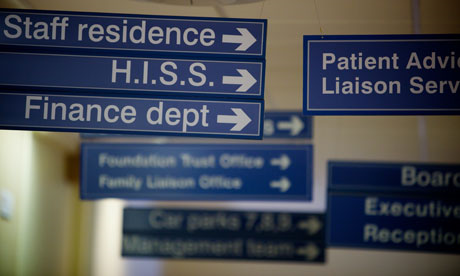
\includegraphics[width=\textwidth]{Alder-Hey-hospital-signs-007.png}
    \caption{Signs placed along a hall. \cite{signs_hospital}} \label{fig:signs1}
  \end{minipage}
  \hfill
  \begin{minipage}{0.45\textwidth}
    \centering
    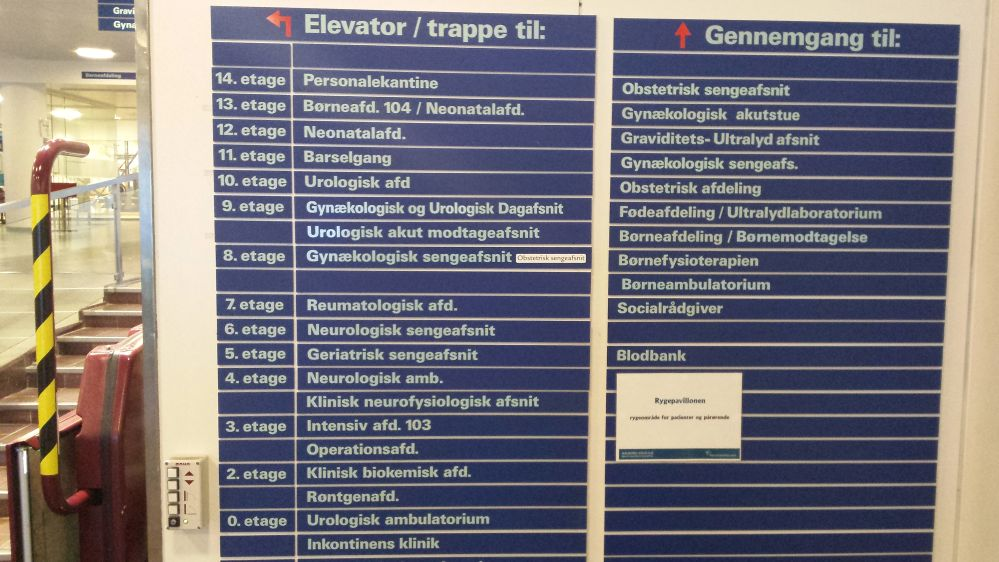
\includegraphics[width=\textwidth]{tavle.jpg}
    \caption{An overview sign of the different floors at Sygehus nord Aalborg} \label{fig:signs2}
  \end{minipage}
  \end{figure}

\subsection{Maps} \label{sub:map}
Analogue maps \cite{map} offer a top-down view of the hospital with all the different locations marked by text or colour \cite{art_Osborne}. See \cref{fig:map}. Maps can be affixed to walls or found in compact versions meant to be carried around. The stationary maps sometimes have a red dot that marks the location of the map. By knowing the current position, the visitor should be able to navigate with more ease \cite{map_survey} as they will not have to look for something recognizable that would otherwise identify their current position. If the building has multiple floors, the map will be split up into layers each depicting a floor in order to more easily represent the 3D structure.

Maps are able to efficiently show hot spots and quickly gain an overview on the location \cite{pros_analog_map}.

A common problem with maps is they can become very complicated to get an overview of if they cover multiple floors \cite{map_confusing}. If the visitor is already inside the building, it can sometimes be difficult to figure out where they are corresponding to the map. If the visitors are in a hallway it can be difficult to distinguish it from the other hallways on the map.

  \begin{figure}[ht!]
  \centering
  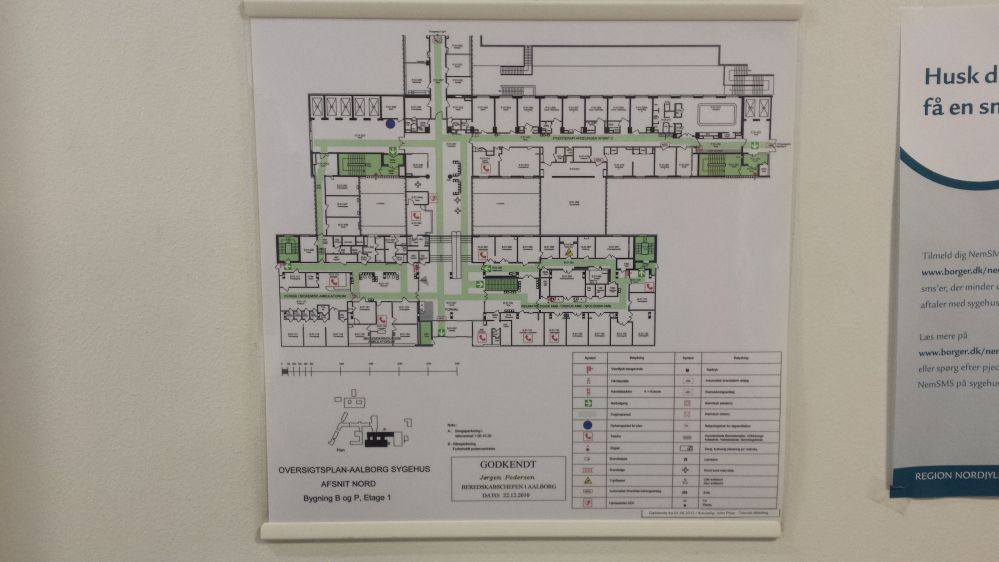
\includegraphics[width=90mm]{kortvaeg.jpg}
  \caption{A map on the wall at Sygehus nord Aalborg}
  \label{fig:map}
  \end{figure}

\subsection{Colour Coding}\label{sub:col}
Coloured stripes are lines painted on walls or floors. See \cref{fig:colour_floor}. They mark key routes to get to certain locations in the hospital. Typically a sign describing the location the colours lead to. One line might say \enquote{recovery} and if followed, will lead to the recovery department. Some departments also have an entire theme in a certain colour. In this way, it might become easier for some people to navigate the next time they visit the hospital, if they can remember the colours representing that department.
Places that use this method of navigation would seamlessly offer an easy way of letting the visitors navigate, because the information provided by the colours are very simple to understand.

A problem with colour coding is that it is very static. If for example some rooms switches their function the stripes on the wall have to be repainted which will be a lot of work. If there are stripes leading to all the different departments, the information could potentially clutch up and become confusing. This method also shares a downside together with the signs, as people with reading disorder  or the colour-blind could have trouble with this form of navigation.

\begin{figure}[htb]
  \begin{center} 
    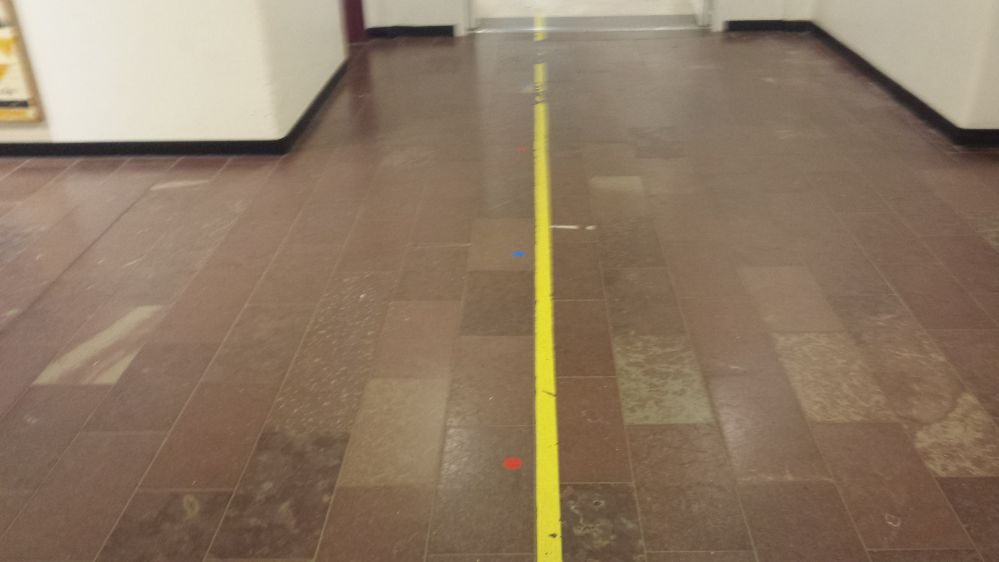
\includegraphics[width=0.5\textwidth]{stribe2.jpg}
  \end{center}
  \caption{Colour coding in use at Sygehus nord Aalborg}
  \label{fig:colour_floor}
\end{figure}




\subsection{Phone}\label{sub:pho}

Visitors are able to call the hospital's main number, and ask questions to a live operator. This can be done from any phone but there is no guarantee that a live operator is available. \cite{sign_ring}
 
The limitations regarding the phone, are high as the informer is limited by only having his/her voice as their tool. Miscommunication can occur as directions only can be delivered by words. As said before, this form of navigation strictly depends on an assigned personal to answer the phone. If no one is at the phone, it becomes utterly useless.
If the service is used often, more than one employee might be assigned to the phone. It could become an expensive service if there is a dedicated staff assigned to the phone.


\subsection{Human Interaction}\label{sub:human}
Visitors can ask the staff including the receptionist regarding navigation around the hospital \cite{job}. Very much like the phone, however human interaction has an advantage of being more precise. There will be less confusion as body language can be used in the answering of the question \cite{body_vs_phone}.

At \enquote{Sygehus Nord Aalborg} a receptionist booth is located at the main entrance. See \cref{fig:rec_booth}. If the visitor arrives at an entrance different from the main one, they might not know where the receptionist is if they need help. The information received from the receptions have to be memorized when the visitor ventures away from the desk. This means that directions could become hard to remember if they have to get to a distant location inside the building. A way the receptionist could help the visitor remember, would be to write a note but even so the text could be misinterpreted or in other ways mixed up.

  \begin{figure}[ht!]
    \centering
    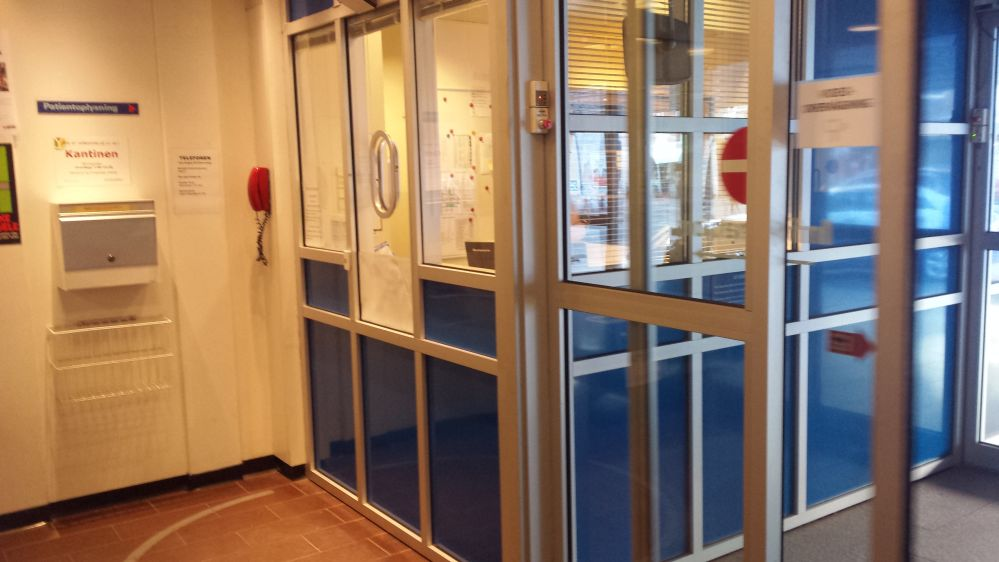
\includegraphics[width=90mm]{reception.jpg}
    \caption{A receptionist booth, seen at Sygehus nord Aalborg}
    \label{fig:rec_booth}
  \end{figure}

\subsubsection{Summary} % (fold)
  We found that in order to have a good navigation platform, the platform needs to be fast to interpret (\cref{sub:sign}), give a fast overview (\cref{sub:map}), be precise (\cref{sub:human}) and easy to understand (\cref{sub:col}). The design of our product has to avoid the weaknesses we have discovered in \cref{sec:anal_nav}. This means that the product must not display irrelevant information (\cref{sub:sign}), must deal with the representation of multiple floors in a non-confusing way (\cref{sub:map}), must deal with positioning without user interaction (\cref{sub:map}), and must be efficient in man hours to maintain (\cref{sub:pho}).